\section{Summary}

To translate the local coordinates defining a 3D model (as exported from tools like Blender) into pixel positions on screen, five sequential steps must be executed: world transform, view transform, projection, normalization, and screen transform. 
Each step facilitates the transformation of coordinates from one space to another.

The initial three steps (and potentially the final one) can be executed through a matrix-vector product. 
However, Normalization mandates a distinct procedure that cannot be merged with the others.

\subsection{Phases}
The steps needed to have the pixels on screen are: 
\begin{enumerate}
    \item An object is initially modeled in local coordinates $p_M$. 
        Typically, these local coordinates are 3D Cartesian, and they are first converted into homogeneous coordinates $p_L$ by appending a fourth component equal to one. 
        The world transform then transitions the coordinates from local space to global space by multiplying them with the world matrix $M_W$. 
    \item The View transform enables visualization of the 3D world from a specific viewpoint in space. 
        It converts coordinates from global space to camera space using the view matrix $M_V$, often generated using either the look-in-direction or look-at techniques.
    \item The Projection Transform readies the coordinates for display on the screen by executing either a parallel or perspective projection. 
        In the case of parallel projections, it employs a parallel projection matrix $M_{P-ort}$ to convert camera space coordinates to normalized screen coordinates. 
        For perspective projections, a perspective projection matrix $M_{P-persp}$ is utilized. 
        In this scenario, the outcomes are not yet normalized screen coordinates but rather an intermediate space known as clipping coordinates.
    \item In many cases, the world, view, and projection matrices are combined into a single matrix, known as the world-view-projection matrix (MWVP).
        During perspective projections, the Normalization step converts clipping coordinates into normalized screen coordinates. Unlike the other transformations, this step involves converting homogeneous coordinates describing points in clipping space into Cartesian coordinates. 
        Specifically, each coordinate is divided by the fourth component of the homogeneous coordinate vector, and then the last component (which is always one) is discarded.
        This step isn't required in parallel projections because the $M_{P-ort}$ matrix already provides normalized screen coordinates. 
        In this case, it suffices to discard the last component, which should already be one.
    \item  In a typical 3D application, the world-view-projection operation is performed, and the resulting clipping coordinates, which define the primitives to be displayed, are sent to the underlying framework. The video card driver then converts these clipping coordinates, if required, first into normalized screen coordinates and then into pixel coordinates for visualizing the objects. 
        This conversion process is conducted in a manner that is transparent to the end user.
\end{enumerate}
\begin{figure}[H]
    \centering
    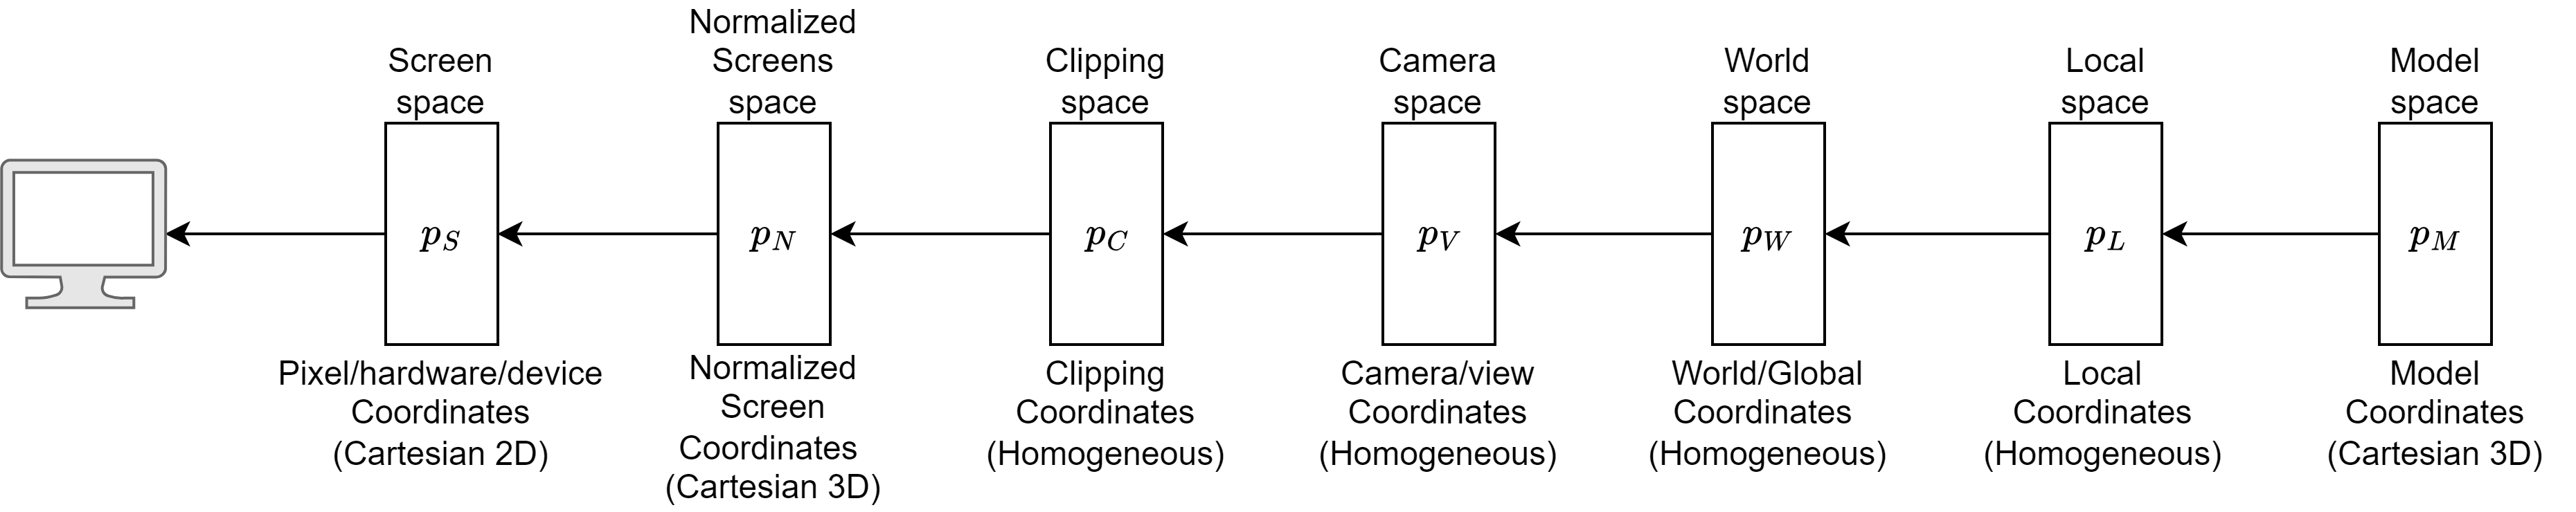
\includegraphics[width=1\linewidth]{images/proj.png}
    \caption{World-view projection matrices}
\end{figure}